\section{Criterio 1: GUTTMAN-KEISER}

Il criterio di Guttman-Keiser per la selezione dei valori singolari da mantenere della SVD troncata prevede di mantenere i valori singolari $\sigma_i$ che sono maggiori di 1:
\begin{equation}
    \sigma_i > 1
\end{equation}
Si tratta dunque di un criterio "oggettivo" in quanto è basato su una soglia numerica ben definita.\\
In questo caso specifico tutti i valori singolari sono maggiori di 1, quindi tutti i valori singolari vengono mantenuti.\\
Il criterio in questo caso, di fatto, si è dunque rivelato inutile.


\begin{table}[H]
    \centering
    \begin{tabular}{|c|c|c|}
        \hline
        \textbf{Matrice} & \textbf{Righe} & \textbf{Colonne} \\
        \hline
        U\_troncata & 301 & 301 \\
        \hline
        S\_troncata & 301 & 301 \\
        \hline
        V\_troncata & 301 & 301 \\
        \hline
    \end{tabular}
    \caption{Dimensioni matrici troncate}
\end{table}

\begin{table}[H]
    \centering
    \begin{tabular}{|c|c|c|}
        \hline
        \textbf{Norma} & \textbf{Errore relativo} & \textbf{Errore assoluto} \\
        \hline
        2 & 0.0 & 0.0 \\
        \hline
        Frobenius & 0.0 & 0.0 \\
        \hline
    \end{tabular}
    \caption{Norme ed errori}
\end{table}

\noindent Dato che tutti i valori singolari sono stati mantenuti, l'errore relativo è nullo.\\
Per la binarizzazione sono state utilizzate le seguenti soglie:
\begin{itemize}
    \item 0.25
    \item 0.5
    \item 0.75
    \item Soglia automatica calcolata con \textbf{graythresh}
\end{itemize}

\begin{figure}[H]
    \centering
     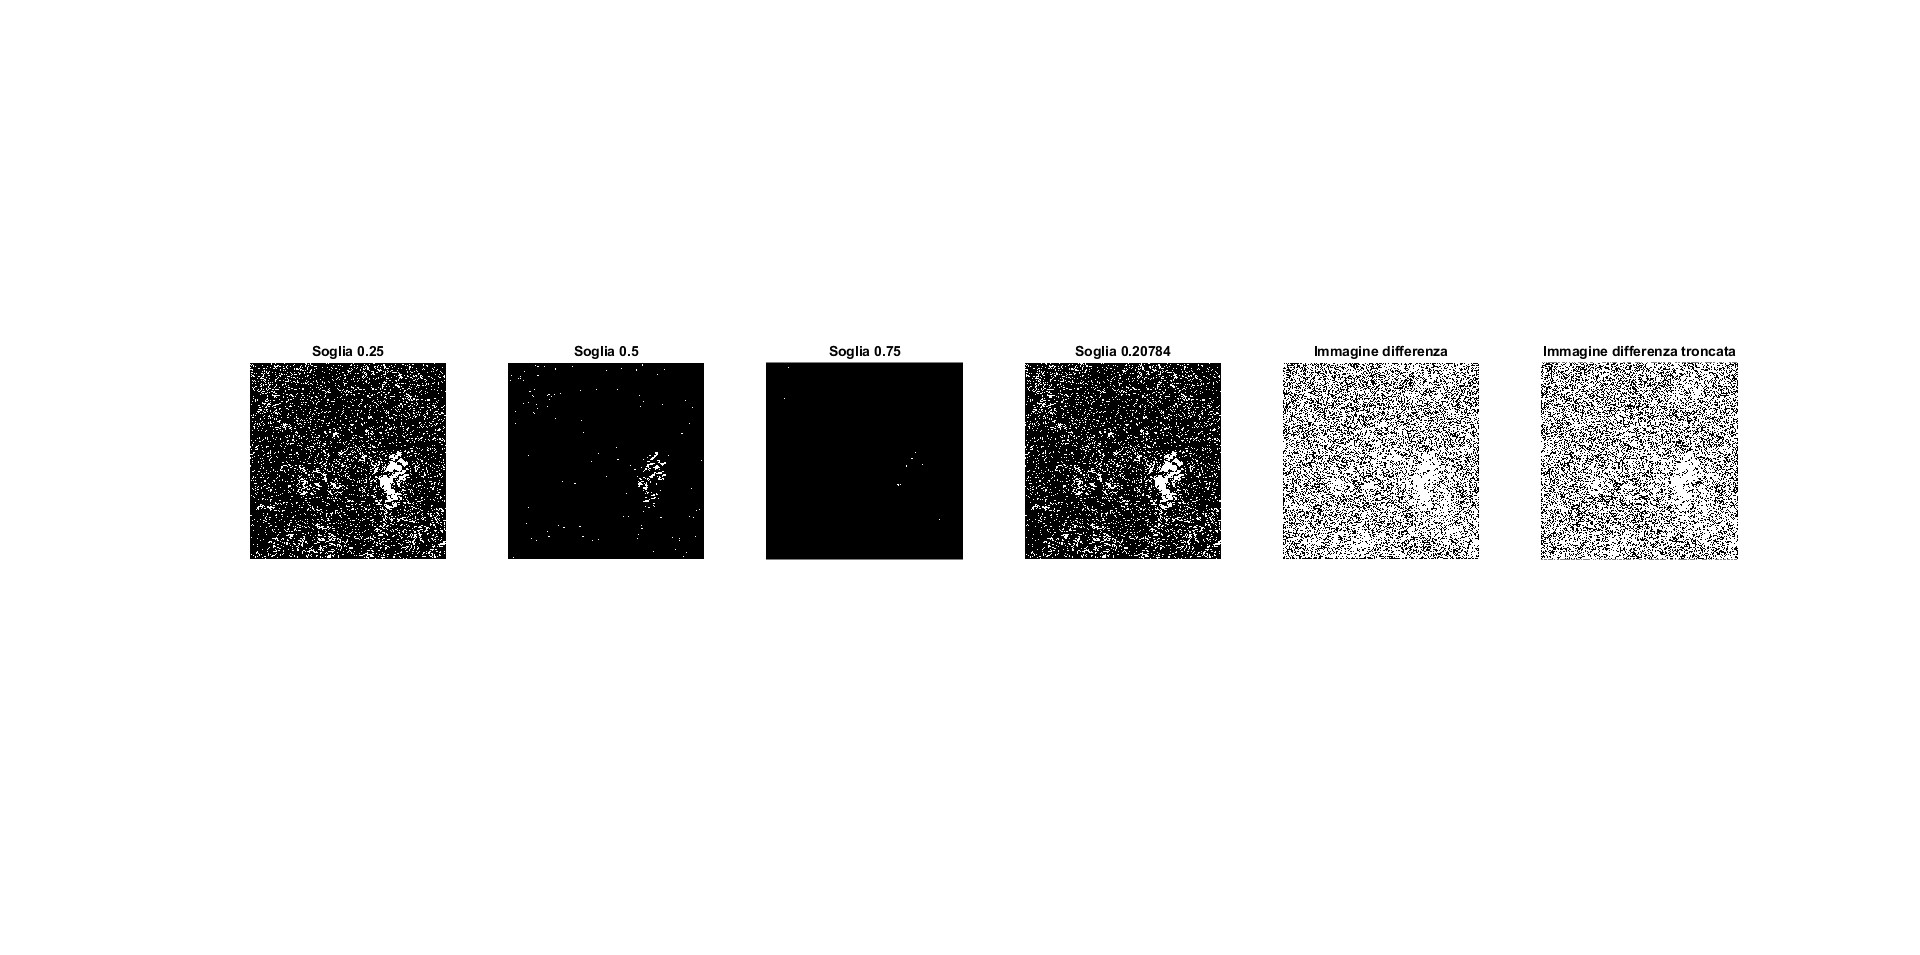
\includegraphics[width=\textwidth]{images/Criterio1.jpg}
    \caption{Immagini binarizzate con criterio 1}
\end{figure}

\noindent Come è possibile notare, ovviamente, in questo caso non vi è differenza tra l'immagine originale e quella approssimata.\\
Per quanto riguarda la binarizzazione si può notare come le soglie 0.5 e 0.75 abbiano prodootto pessimi risultati, mentre la soglia 0.25 e quella automatica abbiano prodotto risultati migliori.\\
\noindent Per il processo di troncamento sono stati necessari in media circa \textcolor{blue}{\textbf{0.0018}} secondi.\\




